\documentclass[tikz, border=10pt]{standalone}

\usepackage{amsmath}

% 1. Use the standard Computer Modern Sans Serif
\usepackage[T1]{fontenc}
\renewcommand{\familydefault}{\sfdefault}


\begin{document}

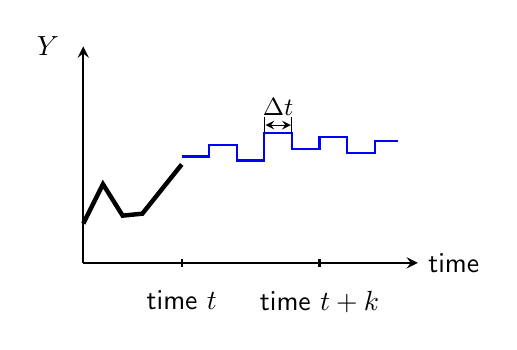
\begin{tikzpicture}[>=stealth, scale=0.5]

    % --- Coordinates ---
    \coordinate (p0) at (0, 0.5);
    \coordinate (p1) at (0.5, 1.5);
    \coordinate (p2) at (1.0, 0.7);
    \coordinate (p3) at (1.5, 0.75);
    \coordinate (p4) at (2.5, 2); % Point at time t

    % --- Axes ---
    \draw[->, thick] (0, -0.5) -- (8.5, -0.5) node[right] {time};
    \draw[->, thick] (0, -0.5) -- (0, 5) node[left=5pt] {$Y$};
    
    % Ticks and Labels
    \draw[thick] (2.5, -0.4) -- (2.5, -0.6) node[below=5pt] {time $t$};
    \draw[thick] (6.0, -0.4) -- (6.0, -0.6) node[below=5pt] {time $t+k$};

    % --- Observed Data (Solid Line) ---
    \draw[ultra thick] (p0) -- (p1) -- (p2) -- (p3) -- (p4);

    % --- Uncertainty Bounds (Dashed Lines) ---
    %\draw[dashed, thick, gray] (p4) to[out=40, in=180] (4.5, 3.5) -- (8, 3.8);
    %\draw[dashed, thick, gray] (p4) to[out=-70, in=180] (4.5, 0.2) -- (8, 0.0);

    % --- Piecewise Constant Forecast (The "Staircase") ---
    % Using -| operator to create steps
    \draw[blue, thick] (2.5, 2.2) 
        -| (3.2, 2.5) 
        -| (3.9, 2.1) 
        -| (4.6, 2.8) 
        -| (5.3, 2.4) 
        -| (6.0, 2.7)
        -| (6.7, 2.3)
        -| (7.4, 2.6) -- (8.0, 2.6);

    % --- Highlight Delta t ---
    % Drawing a small indicator for the step width
    \draw[|<->|] (4.6, 3) -- (5.3, 3) node[midway, above] {\small $\Delta t$};

    % --- Uncertainty Arrow and Question Mark ---
    %\draw[<->, thick] (6, 3.65) -- (6, 0.1) node[midway, right=5pt] {\Large \textbf{?}};

\end{tikzpicture}
\end{document}